\section{Directory Class Reference}
\label{classDirectory}\index{Directory@{Directory}}
{\tt \#include $<$dirview.h$>$}

Collaboration diagram for Directory:\begin{figure}[H]
\begin{center}
\leavevmode
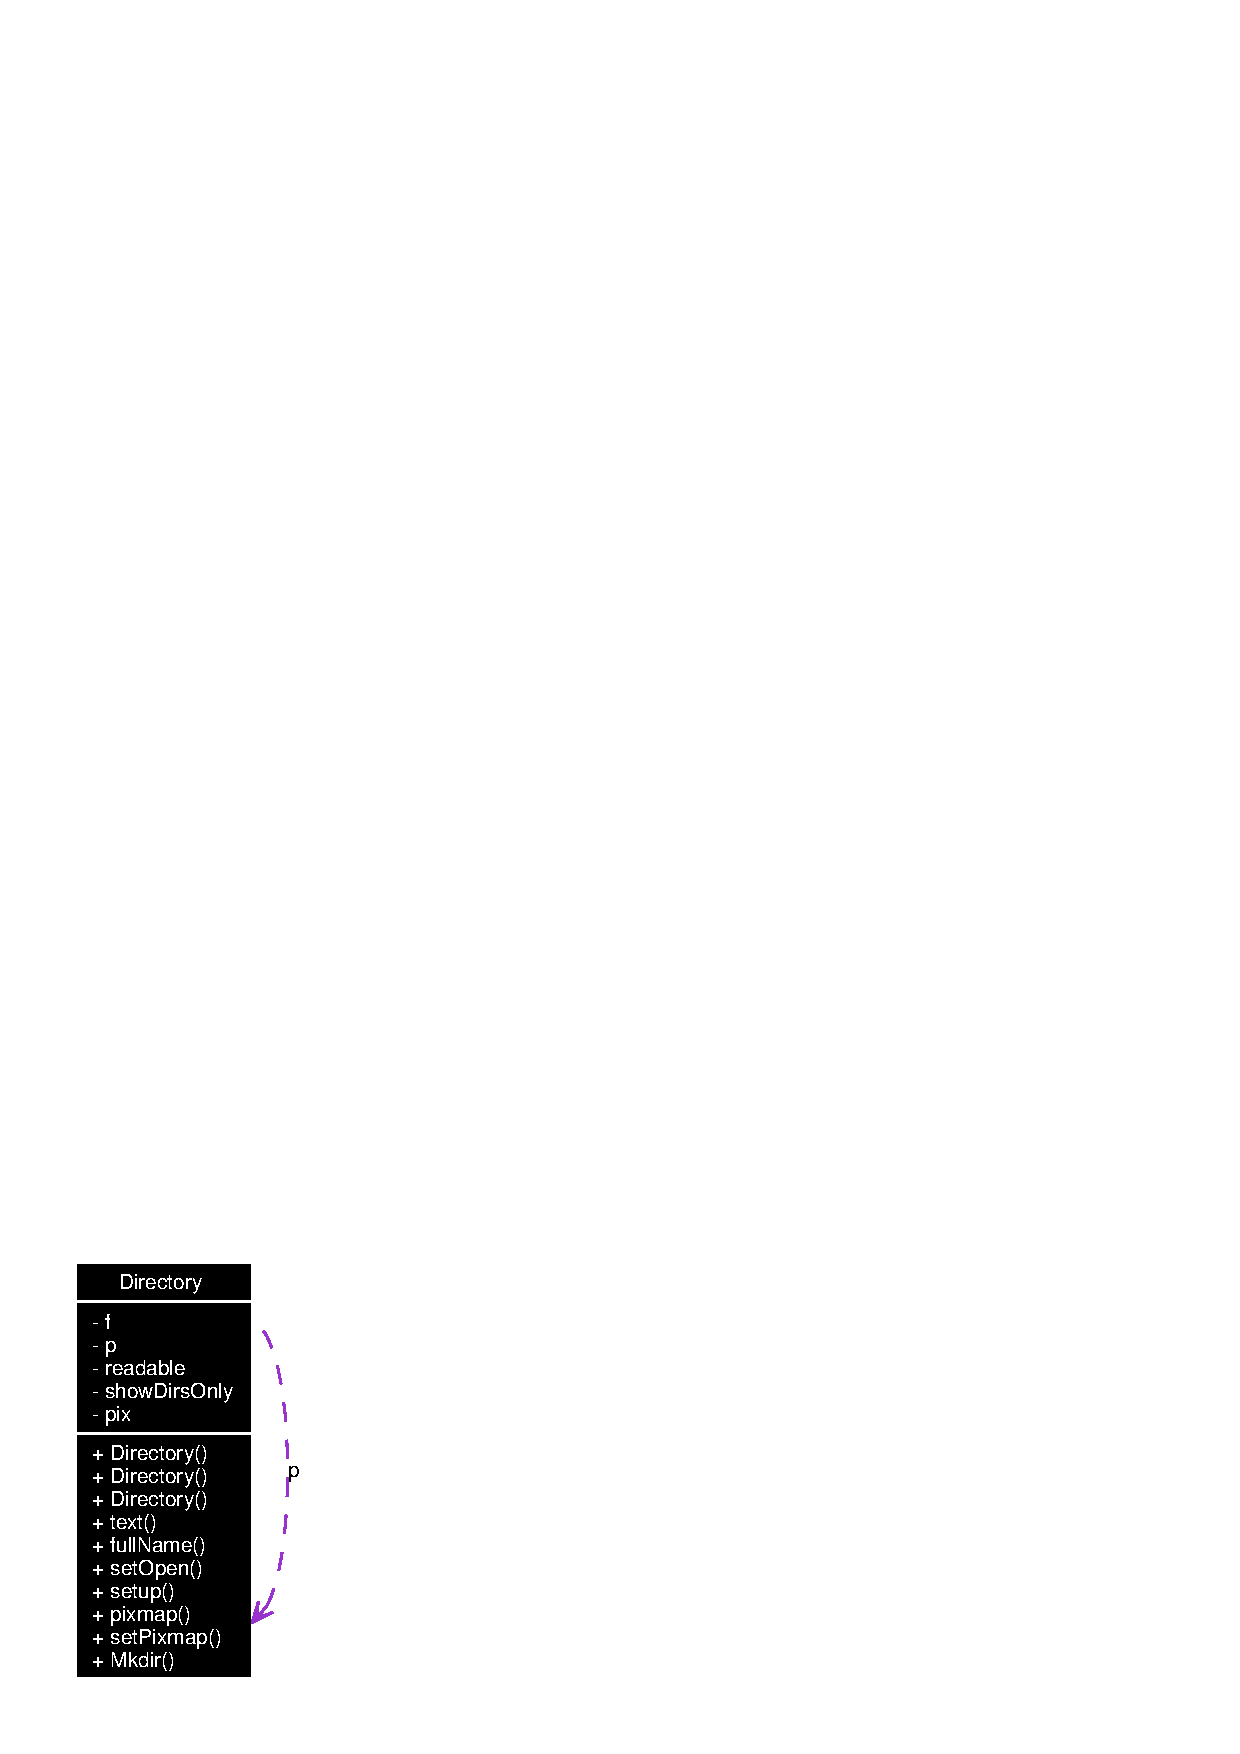
\includegraphics[width=72pt]{classDirectory__coll__graph}
\end{center}
\end{figure}
\subsection*{Public Member Functions}
\begin{CompactItemize}
\item 
{\bf Directory} (QList\-View $\ast$parent, const QString \&filename)
\item 
{\bf Directory} ({\bf Directory} $\ast$parent, const QString \&filename, const QString \&col2)
\item 
{\bf Directory} ({\bf Directory} $\ast$parent, const QString \&filename)
\item 
QString {\bf text} (int column) const 
\item 
QString {\bf full\-Name} ()
\item 
void {\bf set\-Open} (bool)
\item 
void {\bf setup} ()
\item 
const QPixmap $\ast$ {\bf pixmap} (int i) const 
\item 
void {\bf set\-Pixmap} (QPixmap $\ast${\bf p})
\item 
void {\bf Mkdir} (QString s)
\end{CompactItemize}
\subsection*{Private Attributes}
\begin{CompactItemize}
\item 
QFile {\bf f}
\item 
{\bf Directory} $\ast$ {\bf p}
\item 
bool {\bf readable}
\item 
bool {\bf show\-Dirs\-Only}
\item 
QPixmap $\ast$ {\bf pix}
\end{CompactItemize}


\subsection{Constructor \& Destructor Documentation}
\index{Directory@{Directory}!Directory@{Directory}}
\index{Directory@{Directory}!Directory@{Directory}}
\subsubsection{\setlength{\rightskip}{0pt plus 5cm}Directory::Directory (QList\-View $\ast$ {\em parent}, const QString \& {\em filename})}\label{classDirectory_Directorya0}




Definition at line 114 of file dirview.cpp.

References full\-Name(), p, and readable.

Referenced by Mkdir(), and set\-Open().



\footnotesize\begin{verbatim}115     : QListViewItem( parent ), f(filename),
116       showDirsOnly( ( (DirectoryView*)parent )->showDirsOnly() ),
117       pix( 0 )
118 {
119     p = 0;// no parent Directory 
120     readable = QDir( fullName() ).isReadable();
121 
122 }
\end{verbatim}\normalsize 


Here is the call graph for this function:\begin{figure}[H]
\begin{center}
\leavevmode

\includegraphics[width=139pt]{classDirectory_Directorya0_cgraph}
\end{center}
\end{figure}
\index{Directory@{Directory}!Directory@{Directory}}
\index{Directory@{Directory}!Directory@{Directory}}
\subsubsection{\setlength{\rightskip}{0pt plus 5cm}Directory::Directory ({\bf Directory} $\ast$ {\em parent}, const QString \& {\em filename}, const QString \& {\em col2})\hspace{0.3cm}{\tt  [inline]}}\label{classDirectory_Directorya1}




Definition at line 48 of file dirview.h.



\footnotesize\begin{verbatim}49         : QListViewItem( parent, filename, col2 ), pix( 0 ) {}
\end{verbatim}\normalsize 
\index{Directory@{Directory}!Directory@{Directory}}
\index{Directory@{Directory}!Directory@{Directory}}
\subsubsection{\setlength{\rightskip}{0pt plus 5cm}Directory::Directory ({\bf Directory} $\ast$ {\em parent}, const QString \& {\em filename})}\label{classDirectory_Directorya2}




Definition at line 98 of file dirview.cpp.

References folder\-Closed, folder\-Locked, full\-Name(), p, readable, and set\-Pixmap().



\footnotesize\begin{verbatim}99     : QListViewItem( parent ), f(filename),
100       showDirsOnly( parent->showDirsOnly ),
101       pix( 0 )
102 {
103     
104     p = parent;
105     readable = QDir( fullName() ).isReadable();
106 
107     if ( !readable )
108         setPixmap( folderLocked );
109     else
110         setPixmap( folderClosed );
111 }
\end{verbatim}\normalsize 


Here is the call graph for this function:\begin{figure}[H]
\begin{center}
\leavevmode
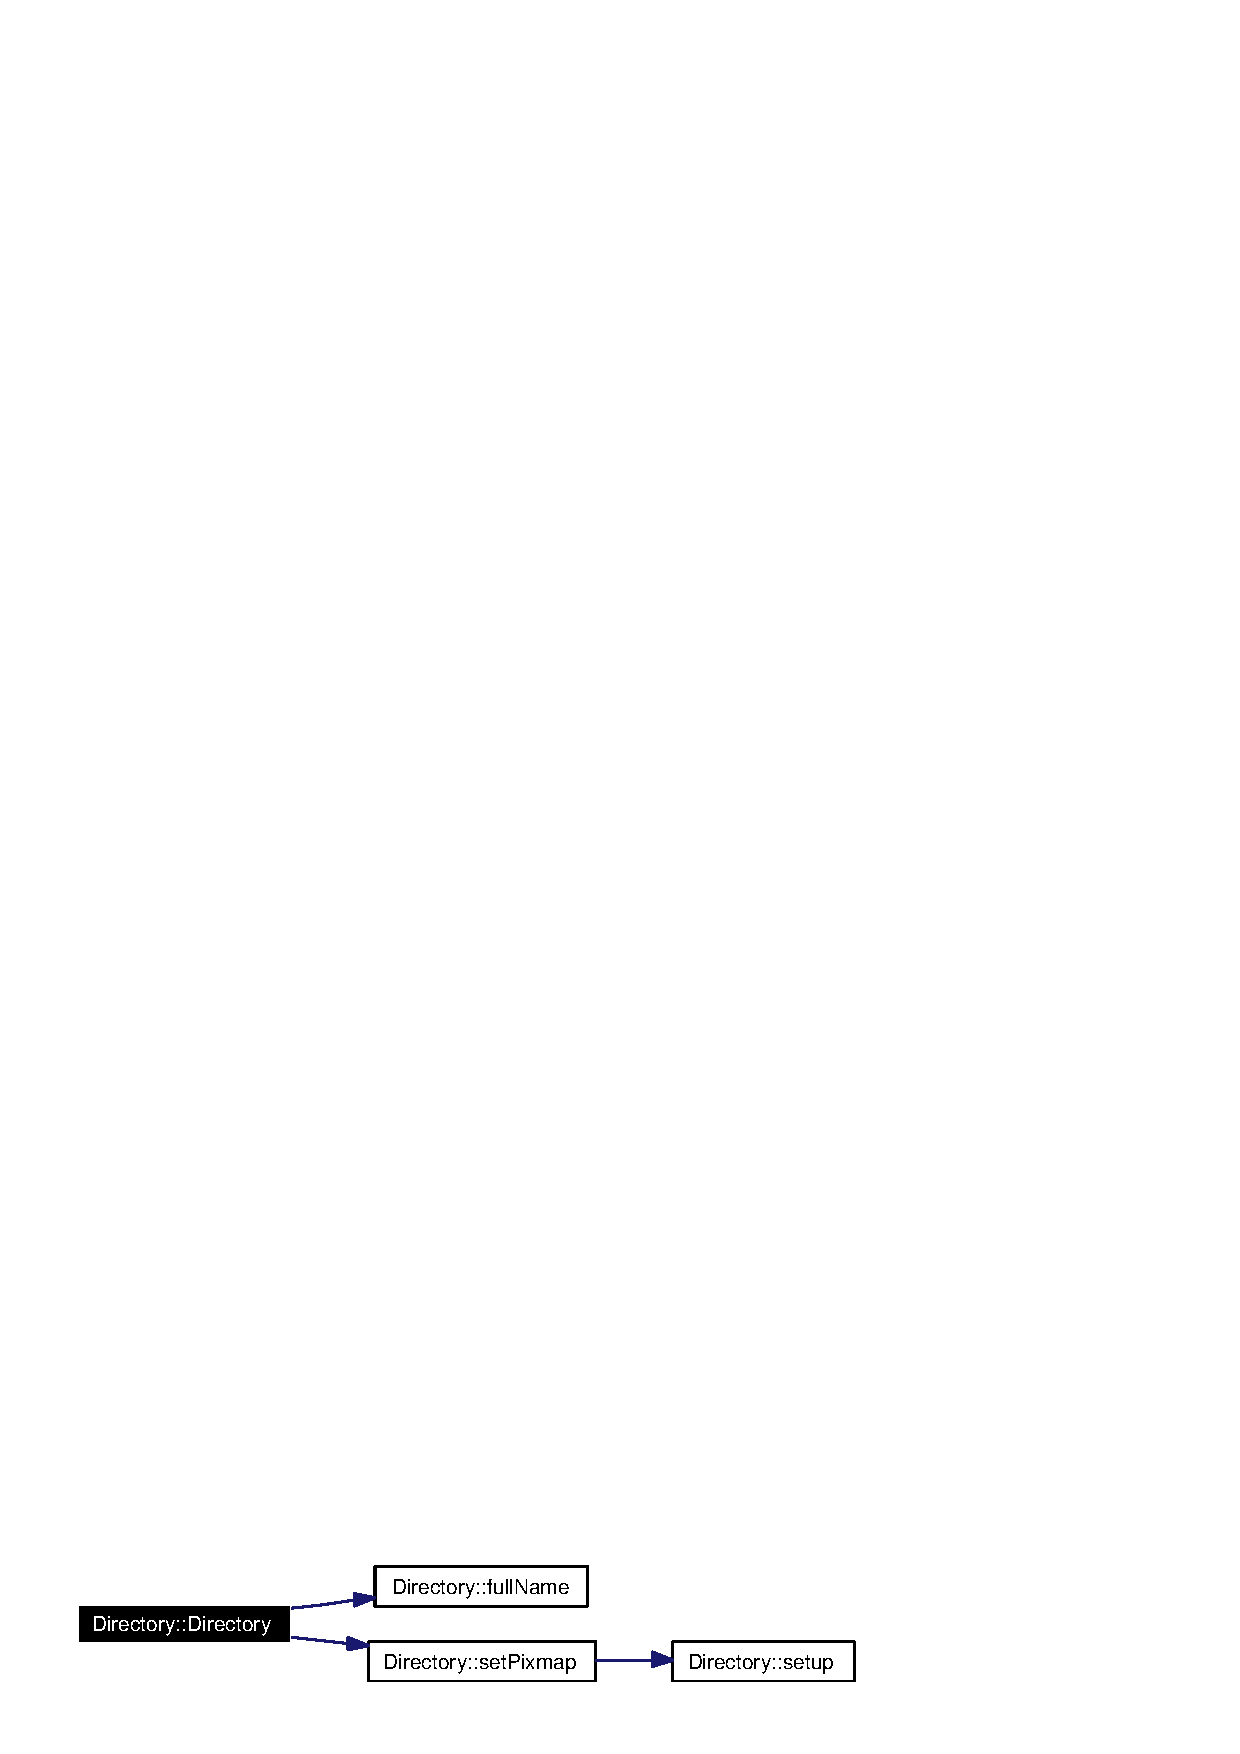
\includegraphics[width=205pt]{classDirectory_Directorya2_cgraph}
\end{center}
\end{figure}


\subsection{Member Function Documentation}
\index{Directory@{Directory}!fullName@{fullName}}
\index{fullName@{fullName}!Directory@{Directory}}
\subsubsection{\setlength{\rightskip}{0pt plus 5cm}QString Directory::full\-Name ()}\label{classDirectory_Directorya4}




Definition at line 199 of file dirview.cpp.

References f, and p.

Referenced by Directory(), Mkdir(), set\-Open(), mediamanagement::slot\-Delete\-Item(), and Directory\-View::slot\-Folder\-Selected().



\footnotesize\begin{verbatim}200 {
201     QString s;
202     if ( p ) {
203         s = p->fullName();
204         s.append( f.name() );
205         s.append( "/" );
206     } else {
207         s = f.name();
208     }
209     return s;
210 }
\end{verbatim}\normalsize 
\index{Directory@{Directory}!Mkdir@{Mkdir}}
\index{Mkdir@{Mkdir}!Directory@{Directory}}
\subsubsection{\setlength{\rightskip}{0pt plus 5cm}void Directory::Mkdir (QString {\em s})}\label{classDirectory_Directorya9}




Definition at line 222 of file dirview.cpp.

References Directory(), and full\-Name().

Referenced by mediamanagement::slot\-Mkdir().



\footnotesize\begin{verbatim}223 {
224         QDir currDir=QDir( fullName() );
225         qWarning(fullName());
226         //DAVID need modified
227         currDir.mkdir(s);
228         new Directory(this,s);
229 }
\end{verbatim}\normalsize 


Here is the call graph for this function:\begin{figure}[H]
\begin{center}
\leavevmode
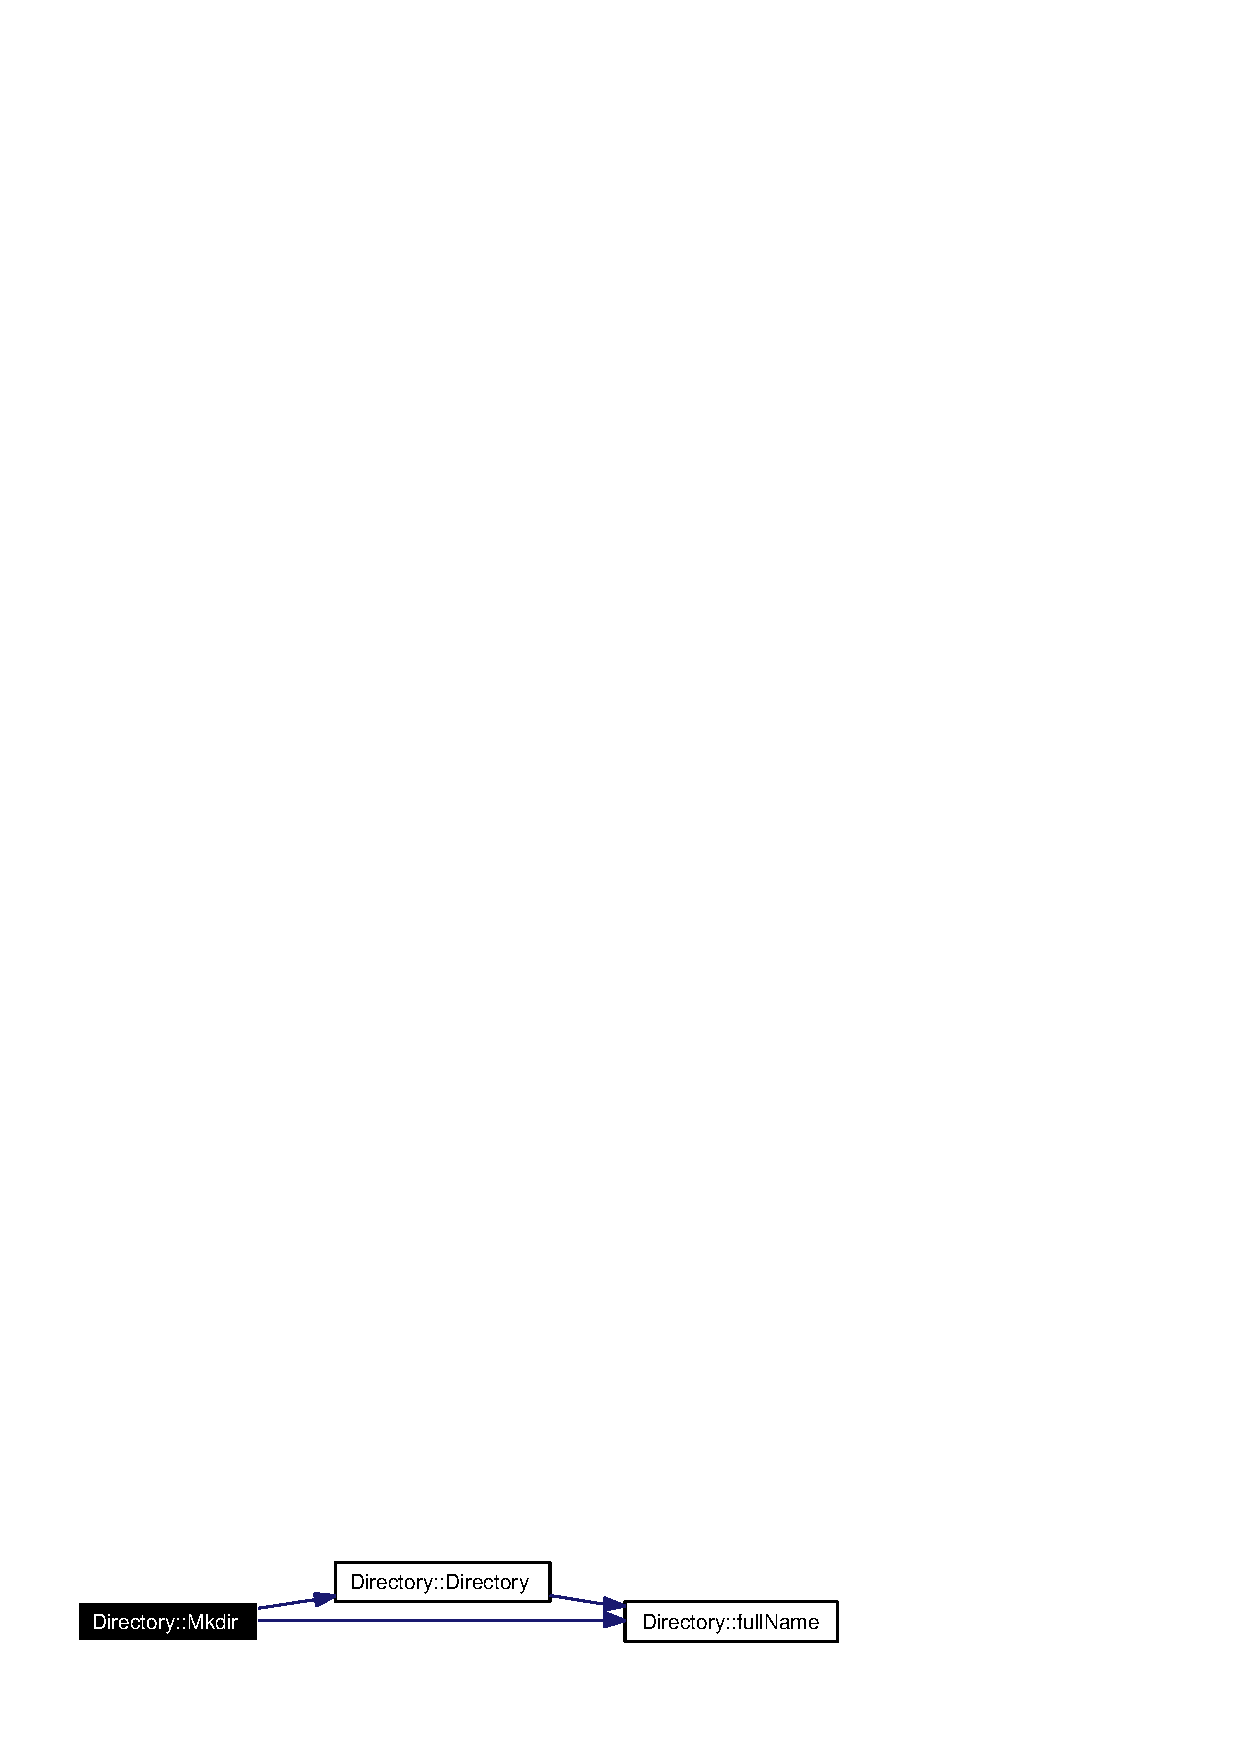
\includegraphics[width=201pt]{classDirectory_Directorya9_cgraph}
\end{center}
\end{figure}
\index{Directory@{Directory}!pixmap@{pixmap}}
\index{pixmap@{pixmap}!Directory@{Directory}}
\subsubsection{\setlength{\rightskip}{0pt plus 5cm}const QPixmap $\ast$ Directory::pixmap (int {\em i}) const}\label{classDirectory_Directorya7}




Definition at line 135 of file dirview.cpp.



\footnotesize\begin{verbatim}136 {
137     if ( i )
138         return 0;
139     return pix;
140 }
\end{verbatim}\normalsize 
\index{Directory@{Directory}!setOpen@{setOpen}}
\index{setOpen@{setOpen}!Directory@{Directory}}
\subsubsection{\setlength{\rightskip}{0pt plus 5cm}void Directory::set\-Open (bool)}\label{classDirectory_Directorya5}




Definition at line 142 of file dirview.cpp.

References Directory(), file\-Normal, folder\-Closed, folder\-Open, full\-Name(), readable, File\-Item::set\-Pixmap(), set\-Pixmap(), and show\-Dirs\-Only.

Referenced by mediamanagement::x\-Setup().



\footnotesize\begin{verbatim}143 {
144     if ( o )
145         setPixmap( folderOpen );
146     else
147         setPixmap( folderClosed );
148 
149     if ( o && !childCount() ) 
150     {
151         QString s( fullName() );
152         QDir thisDir( s );
153         if ( !thisDir.isReadable() ) 
154         {
155             readable = FALSE;
156             setExpandable( FALSE );
157             return;
158         }
159 
160         listView()->setUpdatesEnabled( FALSE );
161         const QFileInfoList * files = thisDir.entryInfoList();
162         if ( files ) {
163             QFileInfoListIterator it( *files );
164             QFileInfo * fi;
165             while( (fi=it.current()) != 0 ) {
166                 ++it;
167                 if ( fi->fileName() == "." || fi->fileName() == ".." )
168                     ; // nothing
169                 else if ( fi->isSymLink() && !showDirsOnly ) {
170                     FileItem *item = new FileItem( this, fi->fileName(),
171                                                      "Symbolic Link" );
172                     item->setPixmap( fileNormal );
173                 }
174                 else if ( fi->isDir() )
175                 {
176                     (void)new Directory( this, fi->fileName() );
177                 }
178                 else if ( !showDirsOnly ) {
179                     FileItem *item
180                         = new FileItem( this, fi->fileName(),
181                                              fi->isFile()?"File":"Special" );
182                     item->setPixmap( fileNormal );
183                 }
184             }
185         }
186         listView()->setUpdatesEnabled( TRUE );
187     }
188     QListViewItem::setOpen( o );
189 }
\end{verbatim}\normalsize 


Here is the call graph for this function:\begin{figure}[H]
\begin{center}
\leavevmode
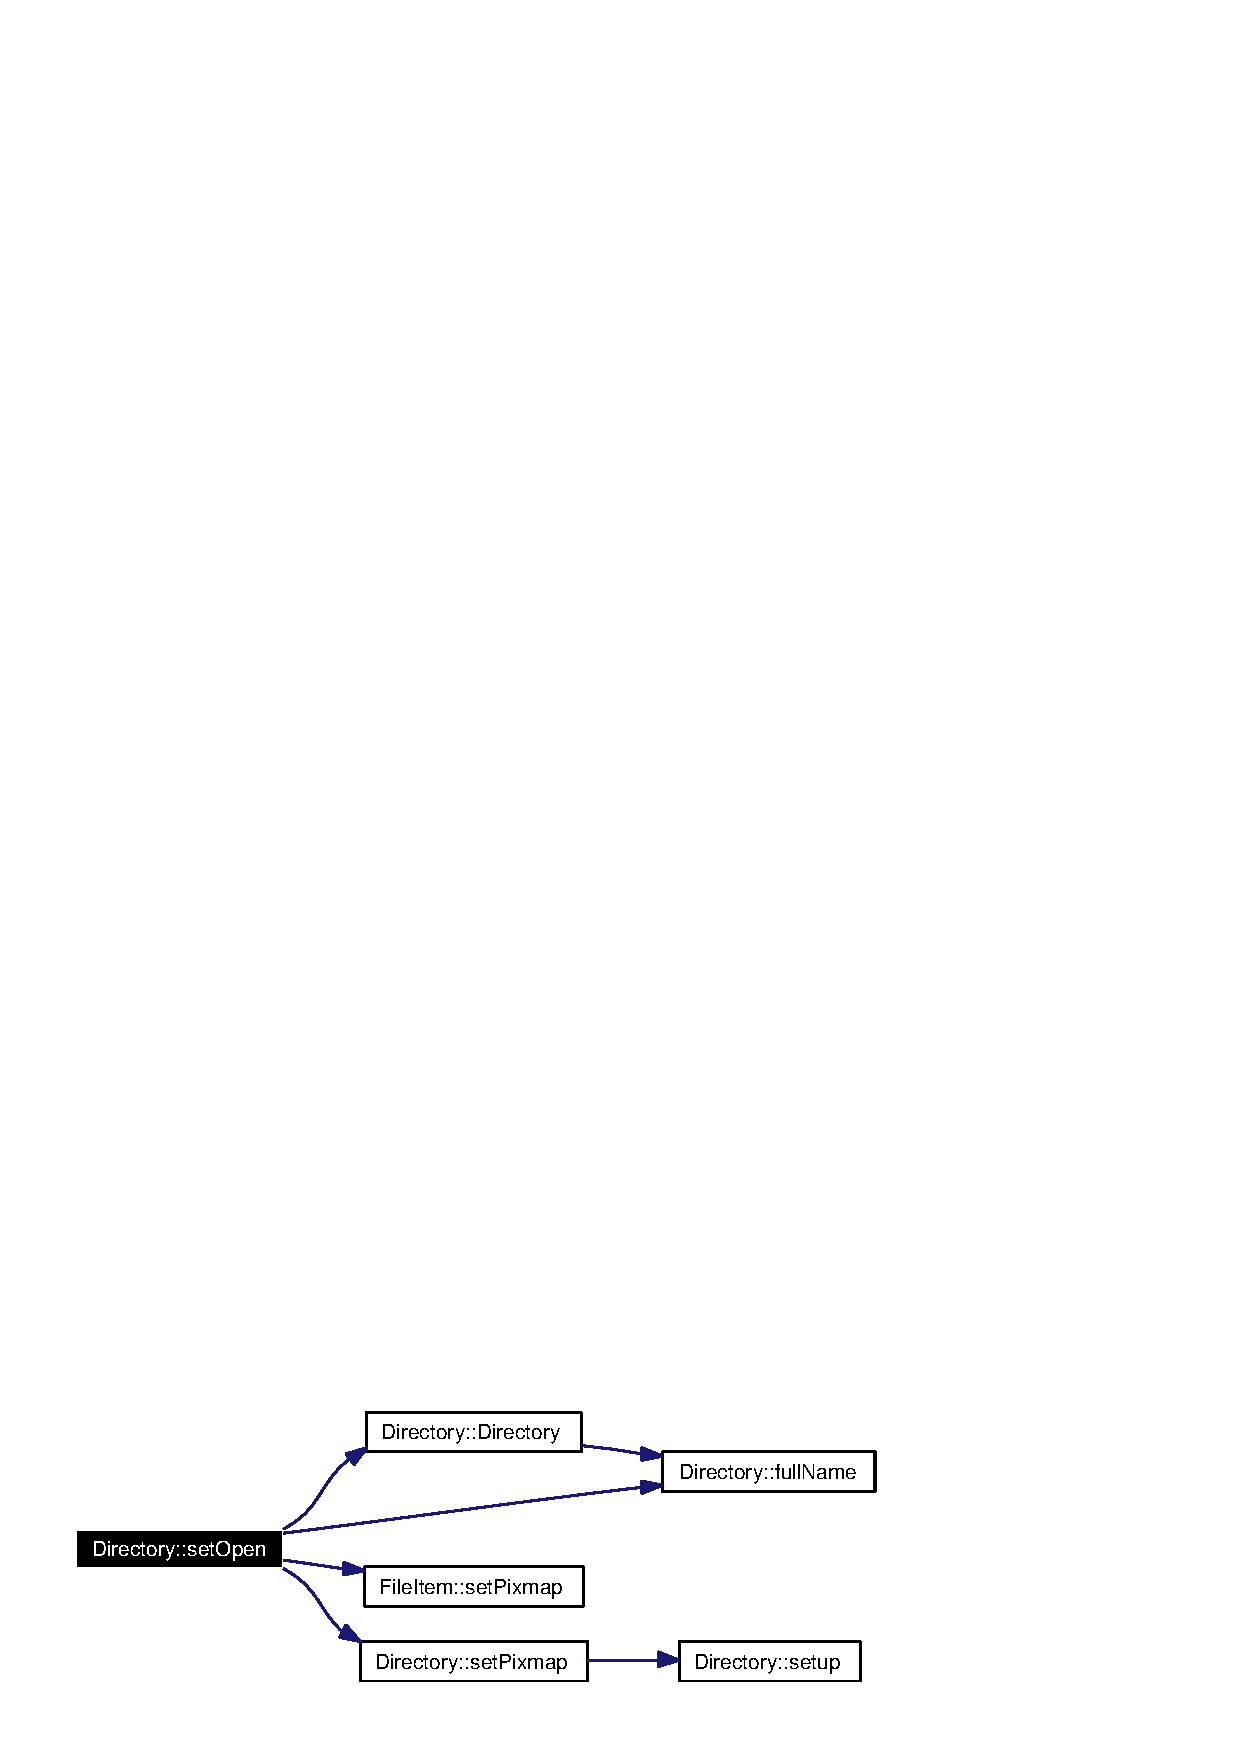
\includegraphics[width=210pt]{classDirectory_Directorya5_cgraph}
\end{center}
\end{figure}
\index{Directory@{Directory}!setPixmap@{setPixmap}}
\index{setPixmap@{setPixmap}!Directory@{Directory}}
\subsubsection{\setlength{\rightskip}{0pt plus 5cm}void Directory::set\-Pixmap (QPixmap $\ast$ {\em p})}\label{classDirectory_Directorya8}




Definition at line 125 of file dirview.cpp.

References setup().

Referenced by Directory(), and set\-Open().



\footnotesize\begin{verbatim}126 {
127     pix = px;
128     setup();
129     widthChanged( 0 );
130     invalidateHeight();
131     repaint();
132 }
\end{verbatim}\normalsize 


Here is the call graph for this function:\begin{figure}[H]
\begin{center}
\leavevmode

\includegraphics[width=135pt]{classDirectory_Directorya8_cgraph}
\end{center}
\end{figure}
\index{Directory@{Directory}!setup@{setup}}
\index{setup@{setup}!Directory@{Directory}}
\subsubsection{\setlength{\rightskip}{0pt plus 5cm}void Directory::setup ()}\label{classDirectory_Directorya6}




Definition at line 192 of file dirview.cpp.

Referenced by set\-Pixmap().



\footnotesize\begin{verbatim}193 {
194     setExpandable( TRUE );
195     QListViewItem::setup();
196 }
\end{verbatim}\normalsize 
\index{Directory@{Directory}!text@{text}}
\index{text@{text}!Directory@{Directory}}
\subsubsection{\setlength{\rightskip}{0pt plus 5cm}QString Directory::text (int {\em column}) const}\label{classDirectory_Directorya3}




Definition at line 213 of file dirview.cpp.

References f, and readable.



\footnotesize\begin{verbatim}214 {
215     if ( column == 0 )
216         return f.name();
217     else if ( readable )
218         return "Directory";
219     else
220         return "Unreadable Directory";
221 }
\end{verbatim}\normalsize 


\subsection{Member Data Documentation}
\index{Directory@{Directory}!f@{f}}
\index{f@{f}!Directory@{Directory}}
\subsubsection{\setlength{\rightskip}{0pt plus 5cm}QFile {\bf Directory::f}\hspace{0.3cm}{\tt  [private]}}\label{classDirectory_Directoryr0}




Definition at line 66 of file dirview.h.

Referenced by full\-Name(), and text().\index{Directory@{Directory}!p@{p}}
\index{p@{p}!Directory@{Directory}}
\subsubsection{\setlength{\rightskip}{0pt plus 5cm}{\bf Directory}$\ast$ {\bf Directory::p}\hspace{0.3cm}{\tt  [private]}}\label{classDirectory_Directoryr1}




Definition at line 67 of file dirview.h.

Referenced by Directory(), and full\-Name().\index{Directory@{Directory}!pix@{pix}}
\index{pix@{pix}!Directory@{Directory}}
\subsubsection{\setlength{\rightskip}{0pt plus 5cm}QPixmap$\ast$ {\bf Directory::pix}\hspace{0.3cm}{\tt  [private]}}\label{classDirectory_Directoryr4}




Definition at line 70 of file dirview.h.\index{Directory@{Directory}!readable@{readable}}
\index{readable@{readable}!Directory@{Directory}}
\subsubsection{\setlength{\rightskip}{0pt plus 5cm}bool {\bf Directory::readable}\hspace{0.3cm}{\tt  [private]}}\label{classDirectory_Directoryr2}




Definition at line 68 of file dirview.h.

Referenced by Directory(), set\-Open(), and text().\index{Directory@{Directory}!showDirsOnly@{showDirsOnly}}
\index{showDirsOnly@{showDirsOnly}!Directory@{Directory}}
\subsubsection{\setlength{\rightskip}{0pt plus 5cm}bool {\bf Directory::show\-Dirs\-Only}\hspace{0.3cm}{\tt  [private]}}\label{classDirectory_Directoryr3}




Definition at line 69 of file dirview.h.

Referenced by set\-Open().

The documentation for this class was generated from the following files:\begin{CompactItemize}
\item 
{\bf dirview.h}\item 
{\bf dirview.cpp}\end{CompactItemize}
